\chapter{Giới thiệu}

\ifpdf
\graphicspath{{Chapter1/Chapter1Figs/PNG/}{Chapter1/Chapter1Figs/PDF/}{Chapter1/Chapter1Figs/}}
\else
\graphicspath{{Chapter1/Chapter1Figs/EPS/}{Chapter1/Chapter1Figs/}}
\fi

Những năm gần đây, \textbf{học tăng cường} (reinforcement learning) liên tục đạt được những thành tựu quan trọng trong lĩnh vực Trí tuệ nhân tạo. 
Những đóng góp nổi bật của học tăng cường bao gồm: tự động điều khiển robot di chuyển, điều khiển mô hình máy bay trực thăng, hệ thống chơi cờ vây ... 
Trong số các thành tựu này, hệ thống chơi cờ vây với khả năng chiến thắng những kỳ thủ hàng đầu thế giới là một cột mốc quan trọng của lĩnh vực Trí tuệ nhân tạo \footnote{\url{https://deepmind.com/alpha-go}}. 
Dù vậy, học tăng cường không phải là một phương pháp mới được phát triển gần đây.
Nền tảng lý thuyết của học tăng cường đã được xây dựng từ những năm 1980 \cite{sutton1998introduction}.

Được xây dựng nhằm mô phỏng quá trình học của con người, ý tưởng chính của học tăng cường là tìm cách lựa chọn hành động tối ưu để nhận được \textbf{nhiều nhất giá trị điểm thưởng} (reward). 
Giá trị điểm thưởng này có ý nghĩa tương tự cảm nhận của con người về môi trường. 
Khi một đứa trẻ bắt đầu ``học'' về thế giới xung quanh của mình, những cảm giác như đau đớn (ứng với điểm thưởng thấp) hay vui sướng (điểm thưởng cao) chính là mục tiêu cần tối ưu của việc học. 
Việc đứa trẻ thực hiện các hành động để tăng cảm giác vui sướng (và giảm đau đớn) cũng tương đồng với việc hệ thống học tăng cường tối đa hoá giá trị điểm thưởng.
Một điểm quan trọng của học tăng cường là các thuật toán được xây dựng với ít giả định nhất có thể về môi trường xung quanh.
Hệ thống sử dụng học tăng cường (agent) không cần biết cách thức hoạt động của môi trường để hoạt động. 
Ví dụ như để điều khiển robot tìm được đi trong mê cung, hệ thống không cần biết mê cung được xây dựng thế nào hay kích thước là bao nhiêu. 
Việc hạn chế tối đa những ràng buộc về dữ liệu đầu vào giúp cho thuật toán học tăng cường có thể áp dụng vào nhiều bài toán thực tế.

Học tăng cường được xem là một nhánh trong lĩnh vực máy học ngoài hai nhánh: \textit{học có giám sát} và \textit{học không có giám sát}. 
Trong bài toán học có giám sát, dữ liệu học thường được gán nhãn thủ công sẵn (hand-labeled); hệ thống cần tìm mối liên hệ giữa dữ liệu và nhãn tương ứng.
Mối liên hệ tìm được sẽ dùng để dự đoán nhãn của dữ liệu mới.
Các nhãn này có thể xem như là sự hướng dẫn trong quá trình học; tính đúng sai của việc học lúc này có thể được xác định dựa vào kết quả dự đoán của hệ thống và nhãn đúng của dữ liệu. 
Tiếp theo đối với những bài toán học không có giám sát, dữ liệu học thường không được gán nhãn nên công việc của việc học là phải tự tìm ra được cấu trúc ``ẩn'' bên dưới dữ liệu đó. 
Khác với hai loại bài toán vừa nêu, trong bài toán học tăng cường, hệ thống không nhận được nhãn thực sự (tức hành động tối ưu của tình huống hiện tại) mà chỉ nhận được điểm thưởng từ môi trường. 
Điểm thưởng lúc này chỉ thể hiện mức độ ``tốt/xấu'' của hành động vừa chọn chứ không nói lên hành động đó có phải là hành động tối ưu hay không. 
Điểm thưởng này thông thường rất \textbf{thưa}: ta có thể chỉ nhận được điểm thưởng có ý nghĩa (khác không) sau hàng trăm hành động. 
Ngoài ra, giá trị điểm thưởng thường không đơn định và rất \textbf{nhiễu}: cùng một hành động tại cùng một trạng thái, ta có thể nhận được điểm thưởng khác nhau vào hai thời điểm khác nhau. 
Hai vấn đề này (tính thưa và nhiễu của điểm thưởng) cũng chính là những khó khăn cơ bản của bài toán học tăng cường.

Game thường hay có điểm số mà người chơi cần phải tối ưu hoá. 
Đặc điểm này trùng với yêu cầu của bài toán học tăng cường, vì vậy game cũng chính là những ứng dụng tự nhiên nhất của phương pháp học tăng cường. 
Trong khoá luận này, chúng em áp dụng phương pháp học tăng cường nhằm xây dựng \textbf{hệ thống tự động chơi các game} trên hệ máy Atari. 
Dữ liệu đầu vào của hệ thống chỉ bao gồm các frame ảnh RGB cùng với điểm số. 
Từ hình ảnh thô này, hệ thống cần tìm cách chơi sao cho điểm số cuối màn chơi (episode) là lớn nhất có thể.
Lưu ý rằng điểm số này được game cung cấp cho hệ thống dưới dạng số thực (chứ không cần phải nhìn hình ảnh thô để ``đọc'' điểm số).
Điểm khó khăn của bài toán này là hệ thống hoàn toàn không biết quy luật của game trước khi bắt đầu quá trình học mà phải tự tìm hiểu quy luật và chiến thuật chơi tối ưu. 
Lý do khoá luận sử dụng game của máy Atari là vì các game này có quy luật chơi tương đối đơn giản nhưng lại rất đa dạng. 
Mỗi màn chơi thường có độ dài vừa phải (từ 2 - 15 phút) và số hành động có ý nghĩa không quá nhiều (18 hành động). 
Ngoài ra, các trò chơi này có thể được giả lập trên máy vi tính với tốc độ cao, giúp quá trình học được tăng tốc.

\begin{figure}
	\centering
	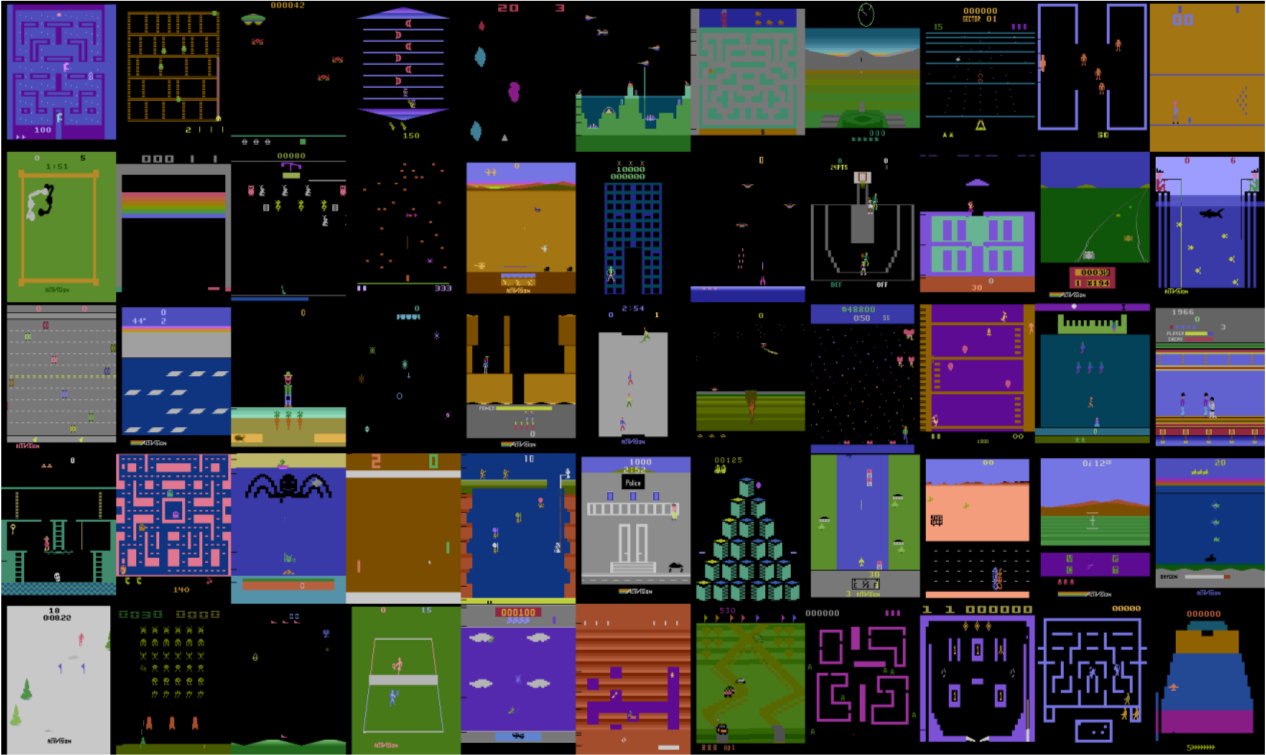
\includegraphics[width=\textwidth]{ale_55_games}
	\caption[Hình ảnh các game trên hệ máy Atari]{Hình ảnh các game trên hệ máy Atari.
	Hình được chỉnh sửa từ \cite{defazio2014comparison}}
	\label{Ale55Games}
\end{figure}

Một số khó khăn trước mắt có thể thấy ở bài toán tự động chơi game bao gồm:
\begin{itemize}
	\item \textbf{Hệ thống không biết luật chơi của game}. 
	Chính vì thế nó cũng không thể biết được hành động nào nên làm hoặc không nên làm ứng với từng tình huống cụ thể.
	\item \textbf{Dữ liệu đầu vào là hình ảnh thô} (ảnh RGB có kích thước $210\times160$). 
	Để học được một chiến thuật chơi đơn giản thì hệ thống cũng phải chơi ``thử và sai'' một số lượng lớn màn chơi (có thể lên đến 10000 frame). 
	Vì vậy, lượng dữ liệu đầu vào cần phải xử lý là rất lớn.
	\item \textbf{Các game rất khác nhau}.
	Khác biệt này là về cả hình ảnh lẫn nội dung của game.
	Để có thể học cách chơi của nhiều game khác nhau thì thuật toán học phải mang tính tổng quát cao, không sử dụng các tính chất riêng biệt của từng game.
	\item \textbf{Chiến thuật chơi game tốt thường phải tính toán dài hạn}.
	Chiến thuật chơi game tốt ở đây mang ý nghĩa đạt được ngang hoặc hơn điểm số mà con người đạt được.
	Những phương pháp tham lam, lựa chọn hành động để đạt điểm tối đa trong tương lai gần thường không đạt được nhiều điểm số.
\end{itemize}

%[TODO: Thêm hướng tiếp cận liên quan + các thực nghiệm + Reference]

%Nhiều phương pháp đã được đề xuất để giải quyết bài toán tự động chơi những game trên hệ máy Atari 2600. Hướng tiếp cận thông thường thường gồm hai giai đoạn [,]. Giai đoạn đầu rút trích đặc trưng từ những frame đầu vào. Trong giai đoạn này ngoài việc chọn ra những đặc trưng tốt cho việc học, nó cũng giúp giảm kích thước dữ liệu đầu vào cho mô hình học. Giai đoạn sau đó thực hiện xấp xỉ hàm 'đánh giá hành động' với đầu vào là những đặc trưng đã rút trích được trong giai đoạn đầu. Nhược điểm của hướng tiếp cận này là mô hình học phức tạp và khó khăn lựa trọn đặc trưng phù hợp cho nhiều game. 
Một trong những tiếp cận đầu tiên cho bài toán tự động chơi game là cuộc thi AAAI General Game Playing được đề xuất từ năm 2005 bởi đại học Stanford \cite{genesereth2005general}.
Trong cuộc thi này, các đội thi nhận được mô tả sơ bộ cho những game được sử dụng để thi.
Các mô hình chi tiết được thiết kế bên dưới các game này không được mô tả cho các đội chơi.
Dựa vào những thông tin nhận được, các đội chơi phải thiết kế một mô hình tổng quát để có thể chơi những game này; trong cuộc thi, họ sẽ chơi ngẫu nhiên một trong những game đã được mô tả \cite{genesereth2005general}.
Đội thắng cuộc trong cuộc thi này đã sử dụng mô hình ``Monte Carlo Tree Search'' (một mô hình phổ biến của học tăng cường) để tìm chiến lược chơi trong những game này.

Trong khoảng ba năm trở lại, tập những game trên hệ máy Atari 2600 trở nên phổ biến trong việc đánh giá khả năng của những phương pháp tiếp cận cho bài toán tự động chơi game.
Những game này bao gồm nhiều thể loại khác nhau như: đối kháng, chiến thuật...
Sự đa dạng trong cách chơi của những game Atari 2600 cùng giao diện lập trình đơn giản làm cho chúng gây được sự chú ý lớn trong cộng đồng Trí tuệ nhân tạo.
Nhiều phương pháp đã được đề xuất liên quan tới bài toán tự động chơi game trên hệ máy Atari 2600. 
Các công trình nghiên cứu như \cite{bellemare2013bayesian, icml2014c2_bellemare14, bellemare2012arcade} chia quá trình học ra thành hai bước.
Bước đầu tiên là hình ảnh game được rút trích đặc trưng bằng các phương pháp rút trích đặc trưng được thiết kế riêng biệt cho bài toán này.
Những phương pháp rút trích đặc trưng này do các nhà nghiên cứu bỏ sức tìm tòi những đặc điểm quan trọng trong bài toán tự động chơi game; các đặc điểm này sau đó sẽ giúp định hướng quá trình thiết kế phương pháp rút trích đặc trưng để lấy được những đặc trưng hữu ích.
Ví dụ như với đặc trưng ``BASS'' \cite{bellemare2012arcade}, đầu tiên hình ảnh game được thực hiện một phép loại bỏ nền (background subtraction).
Hình \ref{fig_bass_feature} mô tả kết quả của phép loại bỏ nền này.
\begin{figure}
	\centering
	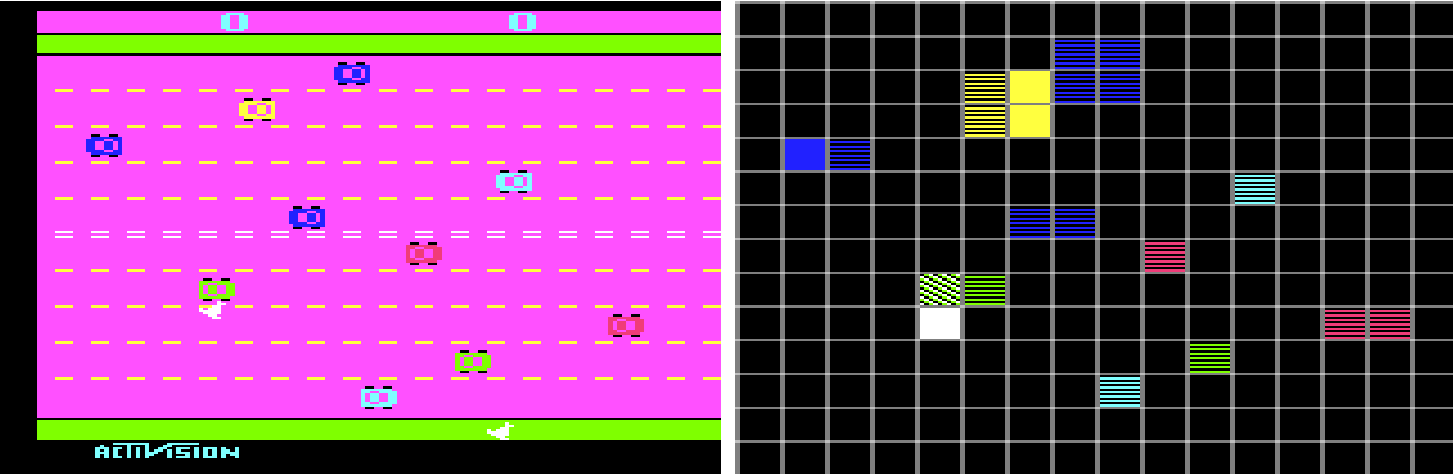
\includegraphics[width=\textwidth]{bass_feature}
	\caption[Phép loại bỏ nền của đặc trưng BASS]{Hình được chỉnh sửa từ \cite{bellemare2012arcade}.
	Hình bên trái là một hình ảnh game gốc trước khi thực hiện loại bỏ nền.
	Hình bên phải là hình ảnh sau khi thực hiện phép loại bỏ nền của đặc trưng ``BASS''.
	}
	\label{fig_bass_feature}
\end{figure}
Bước này giúp việc tìm ra các đối tượng trong hình dễ dàng hơn dựa vào nhận xét là các game Atari thường có hình nền là một màu duy nhất và các đối tượng thường có màu khác.
Tuy nhiên, đặc điểm này chỉ đúng cho các game trên hệ máy Atari nên đặc trưng ``BASS'' rất khó áp dụng cho các game khác.
Đây cũng là điểm yếu chính của các hướng tiếp cận trước đây: việc thiết kế đặc trưng bằng tay rất tốn công sức mà lại không mang tính tổng quát cao.
Bước thứ hai là các đặc trưng này được đưa vào một mô hình học như \textit{``Bayesian learning''} \cite{bellemare2013bayesian} hay \textit{hồi quy tuyến tính} \cite{bellemare2012arcade} để học chiến thuật chơi game.
Tuỳ vào độ phức tạp của đặc trưng đã được rút trích mà người ta chọn thuật toán học tương ứng.
Nếu như đặc trưng học được có kích thước quá lớn thì ta không thể áp dụng các thuật toán học phức tạp hơn được.
Tuy nhiên, thực tế cho thấy, hướng tiếp cận chia quá trình học thành hai bước như thế này tuy phức tạp nhưng lại không cho kết quả tốt \cite{mnih2013playing}.

Vào năm 2015, bài báo \textit{``Human-level control through deep reinforcement learning''} \cite{mnihdqn2015} được công bố trên tạp chí \textit{Nature}.
Bài báo này là của nhóm tác giả Volodymyr Mnih và các cộng sự thuộc nhóm nghiên cứu \textit{Google Deepmind}.
Bài báo này được coi là mở đầu cho những thành công liên tiếp rất lớn trong lĩnh vực Trí tuệ nhân tạo nói chung cũng như trong bài toán tự động chơi game nói riêng.
Sử dụng hướng tiếp cận \textbf{kết hợp học tăng cường với học sâu} (Deep learning), kết quả của bài toán tự động chơi game được cải tiến đáng kể so với những phương pháp cũ (có những game điểm số tăng hơn 20 lần \cite{mnihdqn2015}).
Thay vì chia mô hình học ra thành nhiều phần, hướng tiếp cận này xây dựng một mô hình ``end-to-end'': việc tìm chiến thuật chơi và cách rút trích đặc trưng được học cùng lúc với nhau.
Hướng tiếp cận này giúp đơn giản hoá các vấn đề gặp phải trong những hướng tiếp cận cũ và cải thiện kết quả bài toán.
Cụ thể hơn, nhờ việc áp dụng học sâu, các đặc trưng cần thiết đều được tự động học mà không cần con người tốn sức thiết kế bằng tay.
Ngoài ra, việc xây dựng một mô hình ``end-to-end'' giúp cho quá trình rút trích đặc trưng được gắn liền với việc xây dựng chiến thuật chơi; điều này giúp cho mô hình có khả năng học được những đặc trưng hữu ích cho chiến thuật chơi đó - điều mà các kỹ thuật cũ không thể thực hiện được vì các cách thiết kế đặc trưng đã được cố định trước.
Trong khoá luận này, chúng em tìm hiểu và cài đặt lại mô hình được đề xuất bởi \cite{mnihdqn2015}.
Cùng với đó, chúng em cũng tìm hiểu và cài đặt thêm một mô hình cải tiến của \cite{mnihdqn2015} được đề xuất trong bài báo \cite{van2015deep}.
Mô hình của \cite{mnihdqn2015} gặp phải vấn đề đánh giá quá cao giá trị của các hành động trong game.
Điều này làm cho khả năng chơi của hệ thống bị ảnh hưởng đáng kể (vì hệ thống chọn lựa hành động không tối ưu).
Mô hình cải tiến của \cite{van2015deep} giải quyết vấn đề đánh giá quá cao này và giúp cải thiện đáng kể kết quả của bài toán tự động chơi game.
Ngoài ra, về mặt cài đặt, chúng em thực hiện cài đặt tính toán song song trên GPU (Graphics Processing Unit) để tăng tốc quá trình huấn luyện.

\medskip
Phần còn lại của khoá luận được trình bày như sau:
\begin{itemize}
	\item Chương 2 trình bày kiến thức nền tảng về phương pháp học tăng cường.
	\item Chương 3 trình bày về hướng tiếp cận mà khoá luận tìm hiểu: \textbf{kết hợp học tăng cường với học sâu}.
	Đây là phần chính của khoá luận.
	\item Chương 4 trình bày kết quả thực nghiệm của hướng tiếp cận này cho bài toán tự động chơi game.
	\item Cuối cùng, kết luận và hướng phát triển được trình bày ở chương 5.
\end{itemize}